%!TEX root = ../Main.tex

% -----------------------------------------------------------------------------
\section{Fusion in Practice}
\label{s:Evaluation}

Stream fusion is ultimately performed for practical reasons. We want the fused result program to run faster than unfused source program. Fused result programs like the one in Fig. \ref{fig:Process:Fused} can be lowered directly to a target language, such as Haskell (maybe using Template Haskell), C or LLVM abstract assembly. The details of such lowering surely affect the performance of the final program, but as they are largely unrelated to the fusion algorithm itself, we focus on the form of the fused program expressed directly in the process language.


% -----------------------------------------------------------------------------
\subsection{Fusability}
\label{s:FusionOrder}
When we fuse a pair of processes we commit to a particular interleaving of instructions from each process. When we have at least three processes to fuse, the choice of which two to handle first can determine whether this fused result can then be fused with the third process. Consider our @alternatives@ example from \S\ref{s:EvaluationOrder}, here it is again:
\begin{code}
  alternates : S Nat -> S Nat -> S Nat -> S (Nat, Nat)
  alternates sInA sInB sInC
   = let  s1   = alt2 sInA sInB
          s2   = alt2 sInB sInC
          sOut = zip s1 s2
     in   sOut
\end{code}

In our current system, if fuse the two @alt2@ processes together first, then try to fuse this result process with the downstream @zip@ process, then this final fusion transform fails. This happens because the first fusion transform commits to a sequential instruction interleaving where two output values \emph{must} be pushed to stream @s1@ first, before then pushing values to @s2@. As we discussed in \S\ref{s:EvaluationOrder}, the downstream @zip@ process needs to pull single values from @s1@ and @s2@ alternatively.

Dynamically, if we were to try to execute the result process and the downstream @zip@ process concurrently, then the execution would deadlock. Statically, when we try to fuse the result process with the downstrem @zip@ process then the deadlock is discovered and fusion fails. Deadlock happens when neither process can advance to the next instruction, and in the fusion algorithm this will manifest as the failure of the $tryStepPair$ function from Fig.\ref{fig:Fusion:Def:StepPair}. The $tryStepPair$ function determines which of the instructions from either process can be executed next, and when execution is deadlocked there are none.

On the upside, fusion failure is easy to detect. It is also easy to provide a report to the client programmer that describes why two particular processes could not be fused. The report is phrased in terms of the process definitions visible to the client programmer, instead of partially fused intermediate code. The joint labels used in the fusion algorithm represent which states each of the original processes would be in during a concurrent execution, and we provide the corresponding instructions as well as the abstract states of all the input channels. This reporting ability is \emph{significantly better} than that of prior fusion systems such as Repa~\cite{lippmeier2012:guiding}, as well as the co-recursive stream fusion of \cite{coutts2007stream}, and may other systems based on general purpose program transformations. In such systems it is usually not clear whether the fusion transformation even succeeded, and debugging why it might not have succeeded involves spelunking\footnote{def. spelunking: Exploration of caves, especially as a hobby. Usually not a science.} through many pages (sometimes hundreds of pages) of compiler intermediate representations.

In practice, the likelihood of fusion suceeding depends on the particular dataflow network being used, as well as the form of the processes in that network. For fusion of pipelines of standard combinators such as @map@, @fold@, @filter@, @scan@ and so on, fusion always succeeds. The process implementations of each of these combinators only pull one element at a time from their source streams, before pushing the result to the output stream, so there is no possiblity of deadlock. Deadlock can only happen when multiple streams fan-in to a process with multiple inputs, such as with @merge@. When the dataflow network has a single output stream then we use the method of starting from the process closes to the output stream, walking to towards the input streams, and fusing in successive processes as they occur. This allows the interleaving of the intermediate fused process to be dominated by the consumers, rather than producers, as consumers are more likely to have multiple input channels where need to be synchronized. In the worst case the fallback approach is to try all possible orderings of processes to fuse, assuming the client programmer is willing to wait for the search to complete. 

% We discuss other possible approaches in \S\ref{s:Future:FusionOrder}. 


% When the two @alt2@ processes are fused we end up with a sequential result process. Trying to then fuse that result into the downstream @zip@ process fails. Alternately, if we were to try to concurrently evaluate the fused result process with the downstream @zip@ process would deadlock because we would reach a state where neither process could advance. To state this again: fusion fails when concurrent evaluation of the two source processes would deadlock.

% The main fusion algorithm here works on pairs of processes.
% When there are more than two processes, there are multiple orders in which the pairs of processes can be fused. The order in which pairs of processes are fused does not affect the output values, but it does affect the access pattern: the order in which outputs are produced and inputs read. Importantly, the access pattern also affects whether fusion succeeds or fails to produce a process. In other words, while evaluating multiple processes is non-deterministic, the act of fusing two processes \emph{commits} to a particular deterministic interleaving of the two processes. The simplest example of this has two input streams, a function applied to both, then zipped together. 



% -----------------------------------------------------------------------------
\subsection{Result Size}
                
\TODO{Discuss the performance of the system. Why this is a good idea. Give graphs that show the number of states is sensible when more processes are fused in.}



% -----------------------------------------------------------------------------
\subsection{Optimisation}
\label{s:Optimisation}
After the algorithm has completed fusing both processes it may be possible to eliminate redundant @jump@, depending on how the affected variables are used by other instructions.

\TODO{Discuss combining jump instructions here. Use this to motivate the need for drop instructions.}

\begin{figure}


% I thought these two looked nicer separately, but let me know if you want them in a single graph
\begin{minipage}[t]{0.4\textwidth}
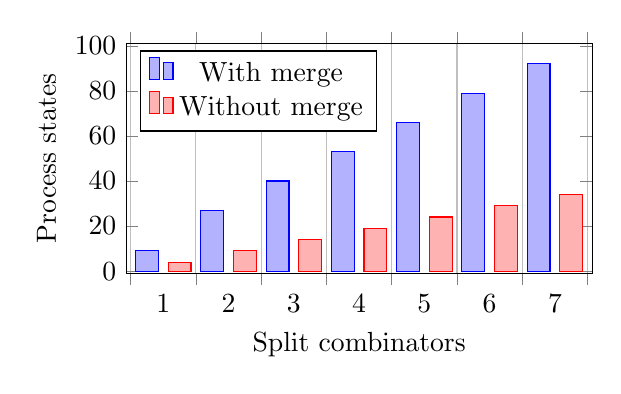
\begin{tikzpicture}
\begin{axis}[
	ylabel=Process states,
	xlabel=Split combinators,
  ymin=0, ymax=100,
	enlargelimits=0.01,
	ybar interval=0.7,
  width=7.5cm, height=4.5cm,
	legend pos=north west,
]
\addplot coordinates {(1,9) (2,27) (3,40) (4,53) (5,66) (6,79) (7,92)
  % Last bar doesn't show for some reason, so need to add a dummy value for the next one
    (8,1) };

\addplot coordinates {(1,4) (2,9) (3,14) (4,19) (5,24) (6,29) (7,34)    (8,1) };

\legend{With merge, Without merge};

\end{axis}
\end{tikzpicture}
\end{minipage}
\begin{minipage}[t]{0.10\textwidth}
\quad
\end{minipage}
\begin{minipage}[t]{0.4\textwidth}
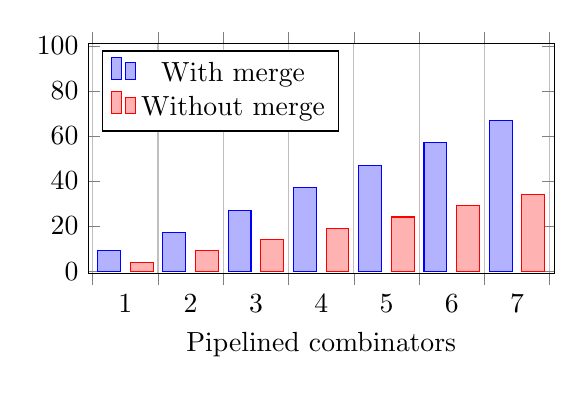
\begin{tikzpicture}
\begin{axis}[
% Hide the label on the second graph
%	ylabel=Process states,
	xlabel=Pipelined combinators,
  ymin=0, ymax=100,
	enlargelimits=0.01,
	ybar interval=0.7,
  width=7.5cm, height=4.5cm,
	legend pos=north west,
]
\addplot coordinates {(1,9) (2,17) (3,27) (4,37) (5,47) (6,57) (7,67)   (8,1) };

\addplot coordinates {(1,4) (2,9) (3,14) (4,19) (5,24) (6,29) (7,34)    (8,1) };

\legend{With merge, Without merge};

\end{axis}
\end{tikzpicture}
\end{minipage}

\caption{Maximum output process size for fusing all combinations of up to $n$ combinators.}
\label{fig:bench:outputsize}
\end{figure}


\begin{figure}

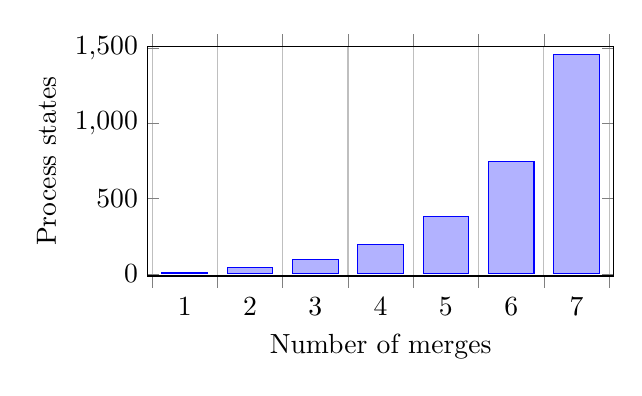
\begin{tikzpicture}
\begin{axis}[
	ylabel=Process states,
	xlabel=Number of merges,
%  ymode=log,
  ymin=0, ymax=1500,
	enlargelimits=0.01,
	ybar interval=0.7,
  width=7.5cm, height=4.5cm,
	legend pos=north west,
]
% These are the values for splitting.
% They are smaller than the 'chaining', but look much nicer on the linear graph.
\addplot coordinates {(1,9) (2,42) (3,97) (4,196) (5,383) (6,746) (7,1461)
  % (8,2880)
  (8,1)
  };

% These are the values for chaining
% \addplot coordinates {(1,4) (2,48) (3,194) (4,760) (5,2814) (6,10064) (7,1) };

\end{axis}
\end{tikzpicture}

\caption{Exponential blowup occurs when splitting or chaining merges together.}
\label{fig:bench:exponential}
\end{figure}

